\section{Considerations on Grain Boundaries}\label{sec:grain-boundaries}

In contrast to free surfaces, where the geometric evolution of a node is not constrained by the surrounding space, in grain boundaries the node shifting acts counter the solid material of the other particle.
This introduces additional constraints, since the grain boundary must not form holes and must not overlap.
The geometric constraints are dependent on the local evolution of the grain boundary nodes, as well as the relative position change of the particles.

Starting from a compact grain boundary, meaning that there are no holes and/or overlap present within it, the condition of maintaining the compactness of the grain boundary can be formulated as follows, if the postions of the particles are fixed.

\begin{align}
    \Step\Shift_\Normal^{|\Parent} = -\Step\Shift_\Normal^{|\Child} \\
    \Step\Shift_\Tangential^{|\Parent} = -\Step\Shift_\Tangential^{|\Child}
    \label{eq:maintain-compact-particles-fixed}
\end{align}

But in reality the positions of particles to each other change, which can be observed macroscopically as shrinkage.
However, the relation between node shifting and particle movement cannot be easily formulated, since the particle movement is effected by the ensemble of all nodes involved in the contact.
But, we can formulate the influence of shifting one single node in normal or tangential direction on the particles' relative postion, if we assume that the other nodes do to hinder movement.
Each contact node has two sets of coordinates, one in the terms of the one particle, one in terms of the other.
However, they represent both the same point in space.

\autoref{fig:model_development/particle_shift_normal} and \autoref{fig:model_development/particle_shift_tangential} show the geometric conditions of such a shift.
The parent particle (index $\Parent$) changes its shape by shifting a single regarded node (green), as the child particle (index $\Child$) also (red).
The particles are assumed to be solely connected in the regarded node, the influence of adjacent nodes is disregarded.
If the new positions of the nodes are put in alignment again, one observes a relative movement of the particles' centers equal to the difference of both node shifting vectors.
This particle center shift leads to a change in contact distance $\Step\Radius_{\Contact} = \Radius'_\Contact - \Radius_\Contact$ and direction $\Step\Angle_\Contact^{|\Parent}$.
The child particle experiences the same direction step as the parent $\Step\Angle_\Contact^{|\Parent} = \Step\Angle_\Contact^{|\Child}$.
The shifting of one node alone does not affect a rotation of the child particle, but the ensemble of node shifts above and below the contact line.
Therefore, the rotation step $\Step\RotationAngle_\Child$ is introduced as another auxiliary variable, whose effect on particle center shift is as in \autoref{fig:model_development/particle_shift_rotation}.

The total movement of the right particle due to node shifting can be formulated as a total differential:
\begin{subequations}
    \begin{align}
        \Step\Radius_\Contact &=
        \frac{\partial \Radius_\Contact}{\partial \Shift_\Normal} \Step\Shift_\Normal
        + \frac{\partial \Radius_\Contact}{\partial \Shift_\Tangential} \Step\Shift_\Tangential
        + \frac{\partial \Radius_\Contact}{\partial \Shift_\RotationAngle} \Step\Shift_\RotationAngle \\
        %
        \Step\Angle_\Contact^{|\Parent} &=
        \frac{\partial \Angle_\Contact^{|\Parent}}{\partial \Shift_\Normal} \Step\Shift_\Normal
        + \frac{\partial \Angle_\Contact^{|\Parent}}{\partial \Shift_\Tangential} \Step\Shift_\Tangential
        + \frac{\partial \Angle_\Contact^{|\Parent}}{\partial \Shift_\RotationAngle} \Step\Shift_\RotationAngle
    \end{align} \label{eq:particle-steps}
\end{subequations}
The partial derivatives therein are obtained from the geometric relations in the above figures.


Of course, for each node the resulting movement of the particle will be different due to geometric relations and diffusive fluxes.
The geometric relations are fixed for a regarded state, but the diffusive fluxes can be used to fulfill \autoref{eq:particle-steps} simultaneously for all nodes involved in a contact.
So there is a set of equations available to describe particle contact conditions as constraints for the TEP-approach.

\subsection{Normal Shifting}

\begin{figure}
    \centering
    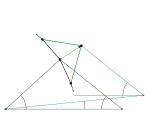
\includegraphics{img/model_development/particle_shift_normal}
    \caption{Effect of Normal Node Shifting on Particle Postion}
    \label{fig:model_development/particle_shift_normal}
\end{figure}

\begin{equation}
    \Step\Shift_\Normal = \Step\Shift_\Normal^{|\Parent} +  \Step\Shift_\Normal^{|\Child}
    \label{eq:contact-ds-normal}
\end{equation}

\begin{equation}
    \eta_\Normal = \PI - \left( \Angle^{|\Parent} - \Angle_\Contact^{|\Parent} \right) + \left( \PI - \SurfaceVectorAngle_\Normal^{|\Parent} - \SurfaceRadiusAngle_\Lower^{|\Parent} \right)
    \label{eq:contact-eta-normal}
\end{equation}

\begin{equation}
    \Radius'_{\Contact} = \sqrt{\Radius_{\Contact}^2 + \Step\Shift_\Normal^2 - 2 \Radius_{\Contact} \Step\Shift_\Normal \cos \eta_{\Normal}}
    \label{eq:contact-rcprime-normal}
\end{equation}

\begin{equation}
    \Step\Angle_{\Contact}^{|\Parent} = \arcsin \left[ \frac{\sin \eta_\Normal}{\Radius'_\Contact} \Step\Shift_\Normal \right]
    \label{eq:contact-dphic-normal}
\end{equation}

\begin{equation}
    \frac{\partial \Radius_\Contact}{\partial \Shift_\Normal}
    = \lim_{\Step\Shift_\Normal \rightarrow 0} \frac{\Radius'_\Contact - \Radius_\Contact}{\Step\Shift_\Normal}
    = - \cos \eta_{\Normal}
    \label{eq:contact-partial-rc-normal}
\end{equation}

\begin{equation}
    \frac{\partial \Angle_\Contact^{|\Parent}}{\partial \Shift_\Normal}
    = \lim_{\Step\Shift_\Normal \rightarrow 0} \frac{\Step\Angle_\Contact^{|\Parent}}{\Step\Shift_\Normal}
    = \frac{\sin \eta_\Normal}{\Radius_\Contact}
    \label{eq:contact-partial-dphi-normal}
\end{equation}

\subsection{Tangential Shifting}

\begin{figure}
    \centering
    \includegraphics{img/model_development/particle_shift_tangential}
    \caption{Effect of Tangential Node Shifting on Particle Postion}
    \label{fig:model_development/particle_shift_tangential}
\end{figure}

\begin{equation}
    \Step\Shift_\Tangential = \Step\Shift_\Tangential^{|\Parent} +  \Step\Shift_\Tangential^{|\Child}
    \label{eq:contact-ds-tangential}
\end{equation}

\begin{equation}
    \eta_\Tangential = - \left( \Angle^{|\Parent} - \Angle_\Contact^{|\Parent} \right) + \left( \PI - \SurfaceVectorAngle_\Tangential^{|\Parent} - \SurfaceRadiusAngle_\Lower^{|\Parent} \right)
    \label{eq:contact-eta-tangential}
\end{equation}

\subsection{Particle Rotation}

\begin{figure}
    \centering
    \includegraphics{img/model_development/particle_shift_rotation}
    \caption{Effect of Particle Rotation on Particle Postion}
    \label{fig:model_development/particle_shift_rotation}
\end{figure}

\begin{equation}
    \Step\Shift_{\RotationAngle} = \frac{\Radius^{|\Child}}{\sin \left(\PI - \Step\RotationAngle_\Child\right)/2} \sin \Step\RotationAngle_{\Child}
    \label{eq:contact-ds-rotation}
\end{equation}

\begin{equation}
    \eta_\RotationAngle = -\left( \Angle^{|\Child} - \Angle_\Contact^{|\Child} \right) + \frac{\PI - \Step\RotationAngle_\Child}{2}
    \label{eq:contact-eta-rotation}
\end{equation}
